\documentclass[a4paper, 12pt,oneside]{book}

% pakiety
\usepackage{polski}
%\usepackage[utf8]{inputenc} % nie można używać as per 
			     % https://tex.stackexchange.com/a/480069/177956
\usepackage{fancyhdr} % nagłówki i stopki
\usepackage{indentfirst} % WAŻNE, MA BYĆ!
\usepackage{graphicx} % to do wstawiania rysunków
\usepackage{amsmath} % to do dodatkowych symboli, przydatne
\usepackage[pdftex,
            left=1in,right=1in,
            top=1in,bottom=1in]{geometry} % marginesy
\usepackage{amssymb} % to też do dodatkowych symboli, też przydatne
\usepackage{pdfpages}
\usepackage{lipsum}
\usepackage{multirow}
\usepackage{listings}
\usepackage{caption}
\usepackage{booktabs}
\usepackage{subcaption}
\usepackage{xcolor}
\usepackage{nameref} % do robienia referencji do chapterów
\usepackage{tikz}
\usetikzlibrary{shapes.geometric, arrows, positioning, angles, quotes}
\graphicspath{ {./img/} }
\DeclareCaptionType{code}[Listing][Spis listingów] 

\definecolor{codegreen}{rgb}{0,0.6,0}
\definecolor{codegray}{rgb}{0.5,0.5,0.5}
\definecolor{codepurple}{rgb}{0.58,0,0.82}
\definecolor{backcolour}{rgb}{0.95,0.95,0.92}

% tikz shapes for flow diagram
\tikzstyle{terminator} = [rectangle, draw, text centered, rounded corners,
                          minimum height=2em]
\tikzstyle{process} = [rectangle, draw, text centered, minimum height=2em]
\tikzstyle{decision} = [diamond, minimum width=2cm, minimum height=0.5,
			text centered, draw=black]
\tikzstyle{data}=[trapezium, draw, text centered, trapezium left angle=60,
                  trapezium right angle=120, minimum height=2em]
\tikzstyle{connector} = [draw, -latex']
\tikzstyle{arrow} = [thin,->,>=stealth]
% tikz shapes for reinforcement learning figure
\tikzstyle{block} = [rectangle, draw, 
    text width=8em, text centered, rounded corners, minimum height=4em]
\tikzstyle{line} = [draw, -latex]
% tikz shapes for Markov chains
\tikzstyle{round}=[thick,draw=black,circle]


\lstset{
	backgroundcolor=\color{backcolour},   
	commentstyle=\color{codegreen},
	keywordstyle=\color{magenta},
	numberstyle=\tiny\color{codegray},
	stringstyle=\color{codepurple},
	basicstyle=\footnotesize,
	breakatwhitespace=false,         
	breaklines=true,                 
	captionpos=b,                    
	keepspaces=true,                 
	numbers=left,                    
	numbersep=5pt,                  
	showspaces=false,                
	showstringspaces=false,
	showtabs=false,                  
	tabsize=2,
	float=h
}

% definicje nagłówków i stopek
\pagestyle{fancy}
\renewcommand{\chaptermark}[1]{\markboth{#1}{}}
\renewcommand{\sectionmark}[1]{\markright{\thesection\ #1}}
% komenda która sprawi że nie numerowany chapter (chapter*) jest dodany do TOC
\newcommand\chap[1]{%
  \chapter*{#1}%
  \addcontentsline{toc}{chapter}{#1}}
\fancyhf{}
\fancyhead[LE,RO]{\footnotesize\thepage}
\fancyhead[LO]{\footnotesize\rightmark}
\fancyhead[RE]{\footnotesize\leftmark}
\renewcommand{\headrulewidth}{0.5pt}
\renewcommand{\footrulewidth}{0pt}
\addtolength{\headheight}{1.5pt}
\fancypagestyle{plain}{\fancyhead{}\cfoot{\footnotesize\thepage}\renewcommand{\headrulewidth}{0pt}}


% interlinia
\linespread{1.25}


% treść
\begin{document}
% strona tytułowa
\sloppy
\thispagestyle{empty}

\includepdf{strona_tytulowa}
\newpage{}

\thispagestyle{empty}
\newpage{}

% spis treści
\tableofcontents{}
\newpage

% pusta strona - narazie zakomentowana
%\thispagestyle{empty}
%\
%\newpage

\chap{Wstęp}
Jedną z większych dziedzin uczenia maszynowego jest uczenie przez wzmacnianie 
(ang. \textit{reinforcement learning}) W odróżnieniu od zarówno uczenia 
nadzorowanego i nienadzorowanego nie potrzebujemy w tym przypadku żadnych
gotowych danych wejściowych i wyjściowych. Zamiast tego, algorytm pozyskuje
dane na bieżąco ze środowiska do, którego jest zastosowany. Dzięki temu,
że algorytmy uczenia przez wzmacnianie nie mają tego ograniczenia możemy
zastosować je do problemów takich jak gra na giełdzie
\cite{trading_reinforcement}, czy nauka grania w gry, w swojej pracy
skupię się na tym drugim.

Celem pracy jest zaimplementowanie algorytmu uczenia przez wzmacnianie\\
Q-Learningu. Następnie zoptymalizowaniu go tak by po zastosowaniu go do
własnoręcznie zaimplementowanej gry był w stanie osiągnąć w niej możliwie
najwyższy wynik. Do zrealizowania tego zostanie użyty język python oraz moduł
pygame.

Na początku przedstawię jaką grę wybrałem, opiszę jej zasady oraz zaprezentuję
szczegóły jej implementacji. Następnie  przybliżę zagadnienie uczenia przez
wzmacnianie oraz algorytmu Q\dywiz learning. Pod koniec pokażę jak
zaimplementowałem wspomniany algorytm, oraz testy po optymalizacjach algorytmu,
które zastosowałem.
\newpage{}

\chapter{Gra}
Problem, który postawiłem przed Q-learningiem to nauczenie się grania w
``Flappy Bird'' -- grę z 2013 autorstwa wietnamskiego developera Dong Nguyena
\cite{flappy_bird_author}. Zdecydowałem się właśnie na tą grę,
gdyż sterowanie w niej jest bardzo proste -- jest tylko jeden przycisk do
kontrolowania toteż jedna akcja do podjęcia przez algorytm.
\section{Zasady gry} 
\begin{figure}[h] 
	\begin{center}
		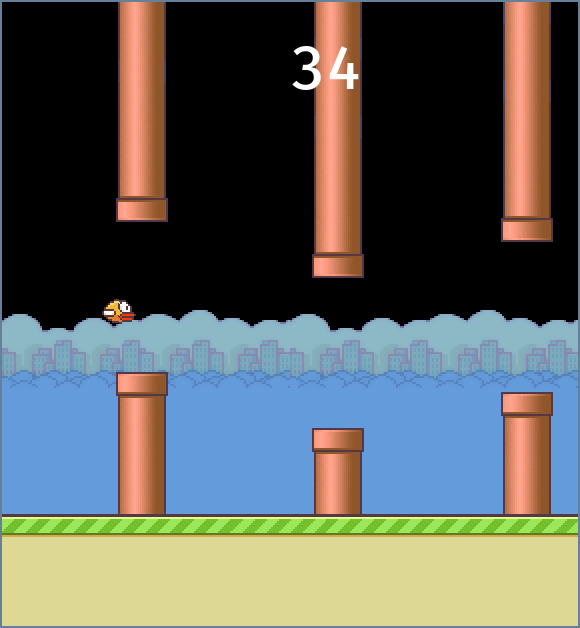
\includegraphics[scale=0.40]{flappy_bird.png}
		\caption{Zrzut ekranu z gry}
		\label{flappy_screenshot}
	\end{center}
\end{figure}

Gracz kontroluje obiekt reprezentowany w grze jako żółty ptak,
jego zadaniem jest tak nim sterować by omijać obiekty reprezentowane przez 
czerwone rury oraz nie pozwolić na to by siła grawitacji doprowadziła do
kolizji obiektu ptaka z obiektem ziemi (na rysunku \ref{flappy_screenshot}
zielona część na dole). Na obiekt ptaka działa jedynie siła grawitacji a
obiekty rur przesuwane są w lewo w jego stronę ze stałą prędkością. Gracz
ma możliwość kontrolować jedynie czy obiekt, którym steruje zwiększy swoją
wysokość o stałą, zakodowaną ilość jednostek czy tego nie zrobi i obiekt
reprezentowany przez ptaka zmniejszy swoją wysokość. Gra kończy się gdy
dojdzie do kolizji obiektu ptaka z, którymkolwiek obiektem rur -- dolnej
bądź górnej albo z obiektem ziemi. Punkty przyznawane są jeżeli graczowi uda
się ominąć nadchodzące przeszkody przelatując przez szczelinę między nimi.
Za każde ominięcie przyznawany jest jeden punkt. Na górze rysunku
\ref{flappy_screenshot} białymi cyframi wypisana jest ilość osiągniętych przez
gracza punktów. Jak widać gracz ominął już trzydzieści cztery pary rur.
Podsumowując -- gra sprowadza się do kontrolowania wysokości ptaka tak by ten
przelatywał między nadchodzącymi rurami.

\section{Wykorzystane technologie}
Do zaimplementowania tej gry zdecydowałem się na użycie wysoko poziomowego
interpretowanego języka \textbf{python} w wersji 3.8. Python jest dostępny na
większości współczesnych platform oraz jest to język  open\dywiz source.
Dodatkowo wykorzystałem moduł \textbf{pygame}.

Pygame dodaje funkcjonalność do biblioteki SDL. Simple DirectMedia Layer(SDL)
jest to wieloplatformowa biblioteka zapewniająca nisko poziomowy dostęp do
audio, urządzeń peryferyjnych takich jak mysz, klawiatura, joystick oraz
sprzętu graficznego (za pomocą OpenGL i Direct3D). Technologia open source
zaimplementowana w C. Używana w grach firm takich jak \textit{Valve Software}
czy \textit{SuperTuxCart}\cite{sdl_ref}. To za pomocą tej biblioteki pygame
może odczytywać wejście czy rysować wyjście na ekranie.

Pygame pozwala tworzyć w pełni funkcjonalne gry oraz programy multimedialne
w pythonie. Zaletami pygame są między innymi : podstawowe funkcje używają
zoptymalizowanego kodu w C oraz Assembly, dostępny podobnie jak python na
większości współczesnych platform. Ponadto jest modularny co pozwala
programiście używać tylko tych komponentów, których naprawdę potrzebuje.
Gier stworzonych z użyciem pygame na samej stronie projektu jest ponad 660
\cite{pygame_about_ref}.
\section{Implementacja}
Głównym elementem implementacji jest nieskończona pętla, w której sprawdzam
zdarzenia, które zaszły, sprawdzam czy mamy wejście od gracza, i aktualizuję
obiekty gry oraz ekran. Na rysunku \ref{game_flow_chart} opisana jako 
\textit{Main game loop}.
\begin{figure}
\begin{center}
\begin{tikzpicture}[node distance = 1.5cm]
\node [terminator] at (0,0) (start) {\textbf{Start}};
\node [process, below of=start] (zainicjalizuj_gre)
{Wczytaj zasoby; zainicjalizuj grę i zegar; zadeklaruj stałe; utwórz grupy};
\node [process, below of=zainicjalizuj_gre] (main_loop) {Main game loop};
\node [decision, below of=main_loop, yshift = -1cm] (900ms) {Minęło $P_f$?};
\node [process, right of=900ms, xshift = 3.5cm] (generate_pipes)
	{Wygeneruj rury};
\node [process, below of=900ms, yshift = -1.7cm] (draw_flappy)
	{Narysuj i zaktualizuj ptaka};
\node [process, below of=draw_flappy] (check_score)
	{Sprawdź czy przyznać punkt};
\node [decision, below of=check_score, yshift = -0.5cm] (check_collision)
	{Kolizja?};
\node [data, below of=check_collision, yshift = -0.9cm] (check_input)
	{Sprawdź input};
\node [decision, below of=check_input, yshift = -0.5cm] (check_esc) {ESC?};
\node [decision, below of=check_esc, yshift = -0.9cm] (check_lpm) {LPM?};
\node [process, right of=check_lpm, xshift = 2.5cm] (flap)
	{Pomachaj skrzydłami};
\node [process, below of=check_lpm, yshift = -0.8cm] (display_update)
	{Zaktualizuj ekran};
\node [terminator, below of=display_update] (end_game) {\textbf{Koniec gry}};
\draw [arrow] (start) -- (zainicjalizuj_gre);
\draw [arrow] (zainicjalizuj_gre) -- (main_loop);
\draw [arrow] (main_loop) -- (900ms);
\draw [arrow] (900ms) -- node[anchor=east] {Nie} (draw_flappy);
\draw [arrow] (draw_flappy) -- (check_score);
\draw [arrow] (check_score) -- (check_collision);
\draw [arrow] (check_collision) -- node[anchor=east] {Nie} (check_input);
\draw [arrow] (check_input) -- (check_esc);
\draw [arrow] (check_esc) -- node[anchor=east] {Nie} (check_lpm);
\draw [arrow] (check_lpm) -- node[anchor=east] {Nie} (display_update);
\draw [arrow] (900ms) -- node[anchor=south] {Tak} (generate_pipes);
\draw [arrow] (check_lpm) -- node[anchor=south] {Tak} (flap);
\draw [arrow] (generate_pipes) |- (draw_flappy);
\draw [arrow] (flap) |- (display_update);
\node [right of = check_collision, xshift = 5cm, inner sep=0pt, outer sep=0pt]
	(phantom_collision) {};
	\draw [arrow] (check_collision) -- node[anchor=south] {Tak}
	(phantom_collision);
\node [right of = check_esc, xshift = 5cm, inner sep=0pt, outer sep=0pt]
	(phantom_esc) {};
\draw [arrow] (phantom_collision) -- (phantom_esc);
\draw [arrow] (check_esc) -- node[anchor=south] {Tak}
	(phantom_esc);
\draw [arrow] (phantom_esc) |- (end_game);
\node [left of = display_update, xshift = -3cm, inner sep=0pt, outer sep=0pt]
	(phantom_display_update) {};
\draw [arrow] (display_update) -- (phantom_display_update);
\draw [arrow] (phantom_display_update) |- (main_loop);
\end{tikzpicture}
\end{center}
\caption{Uproszczony diagram przepływu gry}
\label{game_flow_chart}
\end{figure}
\newpage{}
Program zaczyna od wczytania wczytania zasobów gry -- obrazków reprezentujących
tło, rurę, ziemię, ptaka. Każdemu z tych zasobów tworzy obiekt klasy
\textit{pygame.image}, wczytywane są za pomocą metody \textit{load}.
Do śledzenia czasu w grze wykorzystywany jest obiekt klasy
\textit{pygame.time.Clock}.

Stałe deklarowane na początku programu to na
przykład: ilość jednostek o ile przesunąć w lewo obiekty rur przy każdym
tyknięciu zegara, szerokość szczeliny między obiektami rur, czy czas po jakim
generować nowe rury. W tym miejscu przypisujemy wartość stałej opisującej co
jaki czas mamy generować nowe obiekty rur. Jest wyliczana ze wzoru:
\begin{equation}
	P_f = 900 * (30 \div F)
\end{equation}
Gdzie $P_f$ to czas po jakim generowane są nowe obiekty rur
(ang. \textit{pipe frequency}), $F$ to ilość klatek na sekundę
(ang. \textit{frames per second}). Potrzeba zmiennej częstotliwości
generowania obiektów rur wzięła się z okoliczności, które opisuję w rozdziale
\nameref{chapter:implementacja_qlearningu}.

Przy uruchamianiu programu użytkownik ma opcję wybrać wartość parametru 
klatek na sekundę : 30, 60 bądź 120. Domyślnie jest to 30, stąd we wzorze
znajduje się ta liczba. W ten sposób przy 30 klatkach na sekundę nowe obiekty
rur będą generowane co 900 milisekund, przy 60 co 450 milisekund i co 225
milisekund w przypadku 120 klatek na sekundę. Po kilku próbach stwierdziłem,
że częstsze generowanie obiektów rur sprawiało, że gra była zbyt trudna dla
gracza lub w najgorszym wypadku sprawiało, że gra była nie do przejścia
jak na przykład w scenariuszu przedstawionym na rysunku \ref{frequent_pipes}
gdzie obiekt ptaka nie będzie miał wystarczająco czasu by wznieść się na 
odpowiednią wysokość a potem opaść by ominąć rury. Częstsze generowanie 
obiektów rur nie ma wpływu przy większej ilości klatek na sekundę, gdyż te
przemieszczają się w lewo co tyknięcie zegara o stałą ilość jednostek, a
tykanie zegara uzależnione jest od ilości klatek na sekundę -- większa ilość
klatek na sekundę oznacza częstsze tykanie zegara przez co rury przemieszczają
się z większą prędkością. Rozgrywka staje się zdecydowanie dynamiczniejsza
i przez to również trudniejsza, ale tylko dla ludzi. Q-learningowy agent
dostaje informacje o grze co tyknięcie zegara i jeszcze w tym samym tyknięciu
podejmuje decyzje o ruchu, ale więcej o tym w rozdziale
\nameref{chapter:implementacja_qlearningu}
\begin{figure}
	\begin{center}
		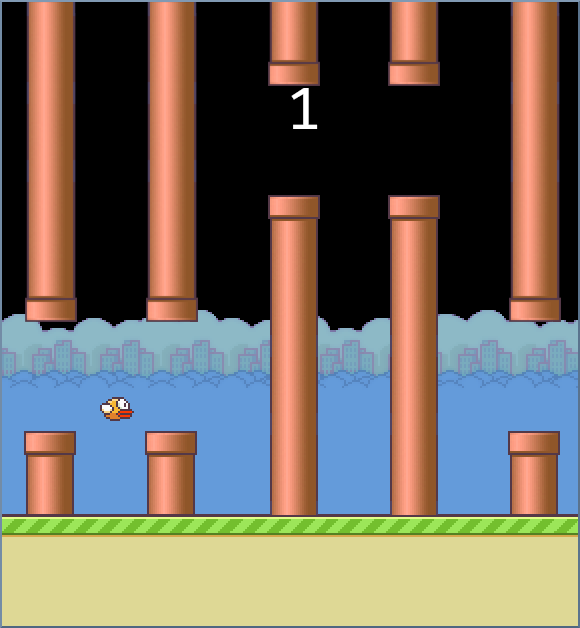
\includegraphics[scale=0.50]{impossible_pipes.png}
		\caption{Często generowane obiekty rur}
		\label{frequent_pipes}
	\end{center}
\end{figure}

Po określeniu wartości stałych tworzymy trzy instancje klasy
\textit{pygame.sprite.Group}, jedną dla obiektu ptaka, drugą dla obiektów rur
dolnych oraz jedną dla obiektów rur górnych. Będą nam potrzebne później przy
sprawdzaniu czy zaszła kolizja między obiektem ptaka a obiektami rur.
Sam obiekt ptaka jest instancją klasy \textit{Bird} dziedziczącej po
\textit{pygame.sprite.Sprite}. Wspomniana klasa jest przeznaczona dla obiektów,
które mają być widoczne na ekranie, zawiera między innymi
pole na obrazek reprezentujący obiekt oraz metodę
\textit{update}\cite{pygame_sprite_documentation}, którą będę wywoływał co
każdy obrót głównej pętli programowej. W przypadku obiektu ptaka w
przeładowanej metodzie \textit{update} znajduje się logika ``latania'' --
co wywołanie metody update inkrementuję zmienną która mówi o ile ma
być przesunięty obiekt ptaka w dół do maksymalnej wartości ośmiu jednostek.
Jeżeli został wciśnięty lewy przycisk myszy to wartość ta jest zmniejszana o
dziesięć (minusowe wartości tej zmiennej powodują, że obiekt zostanie
przesunięty w górę).

Po tym zaczyna się główna pętla programowa. Co $P_f$ czasu generujemy nowe rury
-- polega to na stworzeniu dwóch instancji klasy \textit{Pipe} dziedziczącej
po \textit{pygame.sprite.Sprite}. Generuję liczbę losową $r$ z zakresu
$(-100, 100)$, która będzie potrzebna w ustaleniu wysokości, na której 
wygeneruję obiekty rur. W konstruktorze nadaję obiektom odpowiedni
obrazek. Po wczytaniu obrazku używam \textit{get\_rect}
będącej metodą klasy \textit{pygame.Surface}, której instancją jest nadany w
konstruktorze obrazek. Zwrócony obiekt przypisuję do pola \textit{rect}.
Metoda ta mapuje obrazek na najmniejszy prostokąt, w którym zmieści się
wczytany obrazek. Mamy dzięki temu dostęp do jego krawędzi, którym możemy
nadawać współrzędne na ekranie, w których ma zostać narysowany.
Wszystkie obiekty rysowane są w przestrzeni kartezjańskiej, gdzie punkt
$(0,0)$ jest lewym górnym rogiem tła.
Górnej lewej krawędzi obiektu dolnej rury nadajemy współrzędne:
\[(W, H \div 2 + r + G \div 2)\]
Natomiast dolnej lewej krawędzi obiektu górnej rury nadajemy współrzędne:
\[(W, H \div 2 + r - G \div 2)\]
Gdzie $W$ to szerokość tła ustalona na początku, $H$ to wysokość tła, a
$G$ to stała oznaczająca odległość między dolną a górną rurą, przypisywana
na początku programu. 
Tak narysowane obiekty rur zostaną narysowane zaraz za ekranem z prawej strony,
przesunięte od środku ekranu $x$ oraz połowę odległości ustalonej na początku
działania programu. Tak wygenerowane obiekty dodaję do odpowiednich instancji
\textit{pygame.sprite.Group}. Jako, że klasa \textit{Pipe} dziedziczy po
\textit{pygame.sprite.Sprite} (tak samo jak klasa \textit{Bird}), to powinna
przeładowywać metodę \textit{update}\cite{pygame_sprite_documentation}.
W przypadku klasy reprezentującej rury jest tam tylko logika przesuwania
obiektu w lewo co sprowadza się do zmniejszenia współrzędnej $x$ 
zmiennej \textit{rect} oraz ewentualnym usunięciu go jeżeli współrzędna ta
po zmniejszeniu staje się ujemna (oznacza to, że jest po za lewą krawędzią
ekranu przez co jest nie widoczna i nie potrzebna). Usuwanie polega na
wywołaniu metody \textit{kill}, co powoduje, że obiekt zostaje usunięty
z każdej grupy, której był elementem.

W następnym kroku rysuję na ekranie obiekt ptaka za pomocą metody \textit{draw}
wywoływanej na grupie, do której ten obiekt należy. Metoda ta korzysta z
nadanego w konstruktorze obrazka, oraz zmapowanego obiektu prostokąta
(\textit{sprite.Rect}) do określenia pozycji, na której ma zostać
narysowany\cite{pygame_group_draw_documentation}. Rysowanie obiektów rur odbywa
się w ten sam sposób, z tym, że wspomniana metoda jest wywoływana na
odpowiednio grupie obiektów rur dolnych i górnych. Następnie na grupie, do
której należy obiekt ptaka wywołuję metodę \textit{update}, która obsługuje
logikę ``latania''.

\begin{figure} 
	\begin{center}
		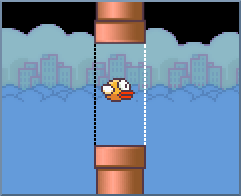
\includegraphics[scale=1.10]{flappy_scoring.png}
		\caption{Granice \textit{rect} obiektów \textit{sprite}}
		\label{flappy_scoring_fig}
	\end{center}
\end{figure}
Najbliższym z prawej strony obiektem rury jest zawsze obiekt o indeksie zero
z grupy dolnych bądź górnych rur, jest tak dzięki logice metody \textit{update}
klasy \textit{Pipe}. Aby sprawdzić, czy przyznać graczowi punkt sprawdzamy
najpierw, czy obiekt ptaka znalazł się w strefie między dwoma rurami, w tym
celu wystarczy sprawdzić czy współrzędna $x$ pola \textit{rect.left} obiektu
ptaka(na rysunku \ref{flappy_scoring_fig} zwizualizowana jako lewa krawędź
czerwonego prostokąta wokół obiektu ptaka) jest większa tej samej współrzędnej
obiektu dolnej rury. Na rysunku \ref{flappy_scoring_fig} jest to zaznaczone
czarną przerywaną linią z lewej strony. Jeżeli tak jest to ustawiam logiczną
flagę reprezentującą to zajście.
W następnych obrotach głównej pętli programowej sprawdzane jest, czy ta flaga
jest ustawiona i jeżeli tak jest to sprawdzam, czy ptak opuścił strefę między
dwoma rurami. Dzieje się to analogicznie do sprawdzania, czy wszedł z tą
różnicą, że porównuję $x$ pola \textit{rect.right} obiektu dolnej rury (to
znaczy współrzędną prawej krawędzi dolnej rury, na rysunku
\ref{flappy_scoring_fig} oznaczona białą przerywaną linią z prawej strony) z
współrzędną $x$ pola \textit{rect.left} obiektu ptaka. Jeżeli tak się stało to
punkt zostaje przyznany a wcześniej wspomnianą flaga zresetowana. Powody
takiego rozwiązania są dwa:
\begin{itemize}
	\setlength\itemsep{-0.4em}
	\item Jeżeli sprawdzałbym tylko czy ptak ominął tylko lewą, albo tylko
		prawą cześć pola \textit{rect} obiektu dolnej rury to punkty
		byłyby naliczane przy każdym obrocie głównej pętli programowej
		gdy obiekt rury najbliższej z prawej został ominięty a nie
		dotarł jeszcze za lewą granicę ekranu i nie został jeszcze
		usunięty.
	\item Jeżeli przyznawałbym punkt, gdy tylko obiekt ptaka znajdzie się
		w strefie między dwoma obiektami rurami to byłaby szansa, że
		gracz wpadnie na obiekt rury zaraz po przyznaniu punktu --
		byłoby to nieprawidłowe zachowanie
\end{itemize}

Aby sprawdzić, czy zaszła kolizja obiektu ptaka z ziemią wystarczy sprawdzić,
czy współrzędna $y$ dolnej części \textit{rect} (czyli \textit{rect.bottom})
będąca zmienną obiektu ptaka jest większa od $H$ (przypomnę, że w
\textit{pygame} układ współrzędnych kartezjańskich ma swój początek w lewym
górnym rogu ekranu a współrzędne z osi $OY$ ``rosną w dół''), gdzie $H$ to
wysokość tła przypisana na początku. Sprawdzenie kolizji między obiektem ptaka
a obiektami rur dzięki \textit{pygame} sprowadza się do wywołania metody
\textbf{pygame.sprite.groupcollide}, która sprawdza, czy doszło do kolizji
pomiędzy dwiema grupami podanymi jako argumenty i zwraca słownik, gdzie
kluczami są obiekty z grupy podanej jako pierwszy argument a wartościami każdy
obiekt z grupy podanej jako drugi argument, z którym obiekt będący kluczem
wszedł w kolizję. Pod spodem metoda ta sprawdza tak naprawdę czy zmienne
\textit{rect} obiektu z każdej grupy nie nachodzą na
siebie\cite{pygame_groupcollide_documentation}. Jako, że grupa
obiektów \textit{Bird} ma tylko jeden element, to wystarczy, że wspomniana
metoda zwróci cokolwiek by stwierdzić, że zaszła kolizja między obiektem ptaka
a obiektami rur i zakończyć grę.

\textbf{Pygame.event} to moduł, który pozwala na interakcję z kolejką wydarzeń,
które odbywają się w systemie np. wciśnięto lub zwolniono przycisk przycisk
myszy bądź klawiatury, zmieniono rozdzielczość ekranu, wyłączono program.
To ten moduł komunikuje się z biblioteką SDL. Jest zależny od modułu
\textbf{pygame.display}\cite{pygame_event_documentation}, który zarządza
wyświetlaniem okna programu na ekranie.
Okno programu jest inicjalizowane na początku działania programu na podstawie
wymiarów obrazków reprezentujących tło i ziemię w grze. Sprawdzanie wydarzeń
polega na iteracji kolejki, którą \textit{pygame} udostępnia za pomocą metody
\textit{pygame.event.get}. Jeżeli zajdzie się w niej wydarzenie o typie
\textit{pygame.QUIT} albo \textit{pygame.KEYDOWN} (został wciśnięty przycisk
klawiatury) oraz \textit{pygame.event.key} to \textit{pygame.K\_ESCAPE}
(wciśnięty klawisz to escape) to podobnie jak w przypadku wykrycia kolizji
gra jest zakańczana.

Dodatkowo \textit{pygame} umożliwia komunikację ze sprzętem bezpośrednio, nie
przez sprawdzanie kolejki wydarzeń. Mysz obsługiwana jest przez moduł
\textbf{pygame.mouse}. Pozwala na sprawdzenie w każdym momencie, które
przyciski na myszy są wciśnięte za pomocą metody
\textit{pygame.mouse.get\_pressed}, która zwraca tablicę wartości logicznych
reprezentujących przyciski na myszy.
Sprawdzenie, czy gracz wcisnął lewy przycisk myszy jest sprawdzane w metodzie
\textit{update} obiektu ptaka i polega na sprawdzeniu dwóch warunków:
\begin{itemize}
	\setlength\itemsep{-0.4em}
	\item Czy lewy przycisk myszy jest wciśnięty
	\item Czy lewy przycisk myszy był wciśnięty w ostatnim obrocie głównej
		pętli programowej
\end{itemize}
Jeżeli przycisk nie był wciśnięty to obiekt ptaka podlatuje i ustawiana jest
flaga logiczna mówiąca o tym, że lewy przycisk myszy jest wciśnięty. Flaga
ta jest resetowana, gdy przy następnym obrocie głównej pętli programowej
przycisk nie będzie wciśnięty. Takie sprawdzanie jest konieczne, inaczej jedno
wciśnięcie lewego przycisku myszy powodowałoby, że obiekt ptaka podlatywał by
do góry o dużą ilość jednostek, dopóki przycisk nie zostałby zwolniony.

Na końcu aktualizowane jest okno gry dzięki użyciu metody
\textbf{pygame.display.update}, która wysyła zaktualizowany obraz na ekran.
Optymalizacja jaka jest zastosowana w tej metodzie, sprawia, że aktualizowane
są tylko te części obrazu, które faktycznie się zmieniły a nie całość.

Gdy gra zostaje zakończona, na ekranie rysowany przycisk reset oraz ustawiana
flaga logiczna zatrzymująca wykonywanie opisanych w tym rozdziale dyrektyw
dopóki nie zostanie wciśnięty lewy przycisk myszy, wtedy gra jest resetowana,
to znaczy wszystkie zmienne są ustawiane do stanu początkowego co powoduje
rozpoczęcie gry na nowo.

\chapter{Uczenie maszynowe}
%Tutaj do napisania o tym czym jest uczenie przez wzmacnianie pare slow jakie są algorytmy
%jak działa, schemat środowisko - agent - akcja - reward\cite{ai_foundations}
\section{Czym jest sztuczna inteligencja}
\textbf{Sztuczna inteligencja} (ang. \textit{artificial intelligence}) to
dziedzina nauki, która zajmuje się syntezowaniem oraz analizowaniem
obliczeniowych agentów, którzy potrafią podejmować inteligentne decyzje.

\textbf{Agent} jest czymś, co potrafi podejmować decyzje w pewnym środowisku,
robić coś. Agentami są na przykład: psy, termostaty, ludzie, korporacje,
samoloty czy roboty.

Mówimy, że agent działa/podejmuje decyzje inteligentnie gdy:
\begin{itemize}
	\setlength\itemsep{-0.4em}
	\item Uczy się na podstawie swojego doświadczenia
	\item Jest elastyczny na zmieniające się środowisko i zmieniające się
		cele
	\item Decyzje, które podejmuje są właściwe dla okoliczności, w których
		się znajduje oraz celów, które ma osiągnąć, biorące pod uwagę
		krótko i długo terminowe konsekwencje
\end{itemize}

\textbf{Obliczeniowy agent} to taki agent, którego podejmowane decyzje mogą
zostać wyjaśnione pod względem obliczeniowym. To znaczy decyzja może zostać
rozbita na podstawowe operacje czyli takie, które mogą zostać zaimplementowane
na fizycznym urządzeniu. Takie obliczenia mogą przyjmować wiele różnych form.
U ludzi są one wykonywane w mózgu, w przypadku komputerów na procesorach.

Wszyscy agenci mają swoje ograniczenia. Żaden agent nie jest wszechmocny czy 
wszechwiedzący. Agenci mogą jedynie obserwować swoje ograniczone środowisko
w bardzo wyspecjalizowanych domenach. Agenci mają skończoną pamięć oraz nie
mają nieskończonej ilości czasu na podjęcie decyzji.

Naukowym celem sztucznej inteligencji jest zrozumienie zasad, które sprawiają,
że inteligentne zachowania są możliwe w naturalnych czy sztucznych systemach.
Jest on osiągany przez:
\begin{itemize}
	\setlength\itemsep{-0.4em}
	\item Analizę naturalnych i sztucznych agentów
	\item Formułowaniem i sprawdzaniem hipotez dotyczących czego potrzeba
		by skonstruować inteligentnych agentów
	\item Projektowanie, budowanie  i eksperymentowanie z systemami
		obliczeniowymi, które wykonują zadania powszechnie uważane
		za wymagające inteligencji
\end{itemize}
Inżynieryjnym celem sztucznej inteligencji jest projektowanie i syntezowanie
użytecznych inteligentnych artefaktów. Chcemy tworzyć agentów, którzy będą
działać inteligentnie. Tacy agenci są użyteczni w wielu problemach.

\section{Interakcja agenta  ze środowiskiem}
Kwintesencją sztucznej inteligencji jest praktyczne rozumowanie, czyli
rozumowanie w celu osiągnięcia jakiegoś celu. Na agenta składa się zespojenie
percepcji, rozumowania oraz podejmowania działań. Agent podejmuje działania w
\textbf{środowisku}.

Agentem może być na przykład komputer z sensorami i siłownikami, innymi słowy
robot, gdzie jego środowiskiem jest świat rzeczywisty. Może być to samo
prowadzący się samochód, lub jak w moim przypadku może być to program, który
działa w czysto obliczeniowym środowisku -- agent programowy (ang.
\textit{software agent}).
\begin{figure}[!htb] 
\begin{center}
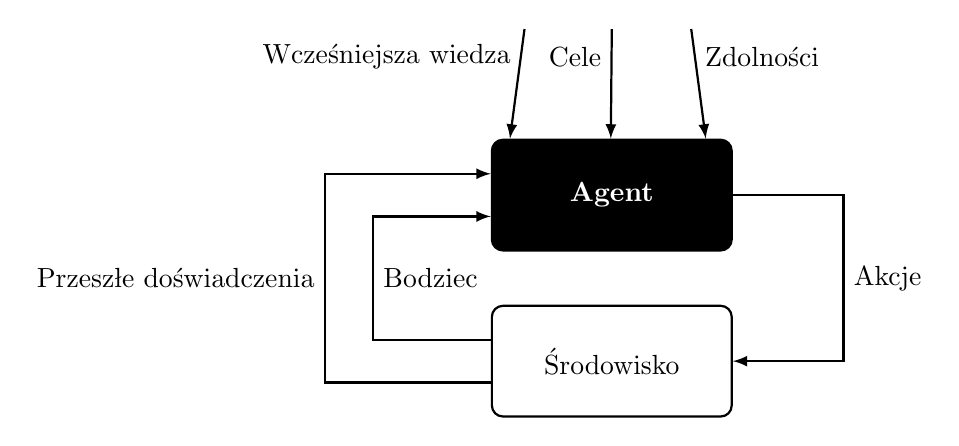
\begin{tikzpicture}[node distance = 6em, auto, thick]
	\node [inner sep=0pt, outer sep=0pt] (Phantom_agent) {};
	\node [left of=Phantom_agent, inner sep=0pt, outer sep=0pt,
		xshift = 1cm] (Phantom_agent_2) {};
	\node [right of=Phantom_agent, inner sep=0pt, outer sep=0pt,
		xshift = -1.1cm] (Phantom_agent_3) {};
	\node [block, below of=Phantom_agent, fill=black, text=white] (Agent)
		{\textbf{Agent}};
	\node [block, below of=Agent] (Environment) {Środowisko};
	\path [line] (Agent.0) --++ (4em,0em) |- node 
	     	[near start]{Akcje} (Environment.0);
	\path [line] (Environment.190) --++ (-6em,0em) |- node
	     	[near start] {Przeszłe doświadczenia} (Agent.170);
	\path [line] (Environment.170) --++ (-4.25em,0em) |- node
	     	[near start, right] {Bodziec} (Agent.190);
	\path [line] (Phantom_agent) --++(0em, 0em) -- node
		[near start, left] {Cele} (Agent.91);
	\path [line] (Phantom_agent_2) --++(0em, 0em) -- node
		[near start, left] {Wcześniejsza wiedza} (Agent.151);
	\path [line] (Phantom_agent_3) --++(0em, 0em) -- node
		[near start, right] {Zdolności} (Agent.31);
\end{tikzpicture}
\end{center}
\caption{Schemat interakcji agenta ze środowiskiem}
\label{rl_figure}
\end{figure}

Rysunek \ref{rl_figure} pokazuje widok czarnej skrzynki agenta z wejściami
i wyjściami. W dowolnym momencie agent jest zależny od:
\begin{itemize}
	\setlength\itemsep{-0.4em}
	\item \textbf{Wcześniejszej wiedzy} o agencie i środowisku
	\item \textbf{Bodźców} otrzymanych od obecnego
		środowiska, które mogą zawierać obserwacje o
		środowisku, ale również akcje, które środowisko
		narzuca agentowi
	\item \textbf{Przeszłych doświadczeń} z poprzednich
		działań i bodźców lub innych danych, z których
		może się uczyć
	\item \textbf{Celów}, które musi starać się osiągnąć
	\item \textbf{Zdolności}, czyli prymitywne działania, które agent
		może wykonać
\end{itemize}
W czarnej skrzynce, agent jest w pewnym stanie wiedzy, może być to wiedza o
środowisku, o tym co próbuje osiągnąć i co zamierza zrobić. Agent aktualizuje
ten stan bazując na bodźcach ze środowiska. Na podstawie stanu wiedzy decyduje
o swoich działaniach\cite{ai_foundations_agents_situated}.

\section{Wiedza agenta} 
W najprostszym przypadku, kiedy agent decyduje co powinien zrobić odnosi się
do modelu środowiska opartego o stany, z celem do osiągnięcia i bez żadnych
niepewności. Agent jest w stanie ustalić jak osiągnąć swój cel przeszukując
przestrzeń stanów środowiska, tak by ze swojego obecnego stanu przejść do
stanu, w którym cel jest osiągnięty. Mając kompletną przestrzeń stanów, próbuje
znaleźć sekwencję działań, których podjęcie sprawi, że osiągnie cel, zanim
jakiekolwiek działania podejmie.

\textbf{Przestrzeń stanów} (ang. \textit{state space}) to jedno z ogólnych
sformułowań inteligentnych działań. \textbf{Stan} zawiera wszystkie informacje
potrzebne do przewidzenia efektów danego działania i ustalenia, czy tenże stan
jest potrzebny do osiągnięcia celu. Przeszukiwanie przestrzeni stanów zakłada:
\begin{itemize}
	\setlength\itemsep{-0.4em}
\item Agent ma całkowitą wiedzę o przestrzeni stanów i planuje na przypadek,
	w którym obserwuje, w którym stanie się znajduje -- jest całkowita
	obserwowalność
\item Agent ma zbiór akcji, które mają znane, deterministyczne efekty na
	środowisko
\item Agent może ustalić czy stan spełnia cel
\end{itemize}
\textbf{Rozwiązanie} to sekwencja działań, które przeniosą agenta z jego
obecnego stanu do stanu, który spełnia cel.

\section{Proces decyzyjny}
W poprzednim podrozdziale założyłem, że rozwiązanie to skończona sekwencja
działań, co jednak, jeżeli problem, który agent, musi rozważyć trwający proces
lub nie wie ile działań będzie musiał jeszcze podjąć. Takie problemy nazywane
są \textbf{problemami nieskończonego horyzontu} (ang. \textit{infinite horizon
problems}), gdzie proces może trwać wiecznie, jak na przykład problem grania
we ``Flappy Bird'' lub \textbf{problemami nieokreślonego horyzontu} (ang.
\textit{indefinite horizon problems}), w którym agent w końcu zakończy
podejmowanie działań, ale nie wie kiedy to nastąpi.

Dla trwających procesów, może nie mieć sensu rozważanie użyteczności na końcu
procesu ponieważ agent może nigdy nie dojść do końca. Zamiast tego agent może
otrzymać sekwencję \textbf{nagród} (ang. \textit{rewards}). Te nagrody włączają
koszt działania, oprócz nagród mogą agentowi mogą być nadane również kary.
Negatywne nagrody nazywane są \textbf{karami} (ang. \textit{punishments}).
Problemy niezdefiniowanego horyzontu mogą być wymodelowane używając stanu
stop. \textbf{Stan stop} bądź \textbf{stan absorbujący} to stan, w którym
wszystkie działania nie mają żadnego efektu to znaczy jeżeli agent znajdzie
się w tym stanie to wszystkie jego działania wracają do stanu z zerową nagrodą.
Osiągniecie celu może być wymodelowane w ten sposób, by agent otrzymał nagrodę
właśnie, kiedy osiągnie stan stopu.

\subsection{Łańcuchy Markova}
% http://artint.info/2e/html/ArtInt2e.Ch8.S2.html
Mówimy, że zmienna $X$ jest \textbf{warunkowo niezależna} od losowej zmiennej
$Y$ zakładając, że mamy zbiór losowych zmiennych $Z_s$ jeżeli
\[P(X | Y, Z_s) = P(X| Z_s)\]
gdzie prawdopodobieństwa są dobrze zdefiniowane (żadne nie jest równe $0$).
Zapis $P(X| Y, Z_s)$ oznacza prawdopodobieństwo zajścia $X$ pod
warunkiem, że zajdzie $Y$ oraz $Z_s$. To oznacza, że dla każdego $x \in
\text{dziedzina}(X)$, dla każdego $y \in \text{dziedzina}(Y)$ oraz dla każdego
$z \in \text{dziedzina}(Z_s)$ jeżeli $P(Y = y \wedge Z_s = z) > 0,$
\[P(X=x|Y=y \wedge Z_s = z) = P(X=x|Z_s = z).\]
To znaczy, mając wartość każdej zmiennej $Z_s$, wiedza o prawdopodobieństwie
$Y$ nie ma wpływu na przekonanie o $X$.

% http://artint.info/2e/html/ArtInt2e.Ch8.S3.html
Pojęcie warunkowej niezależności jest użyte by nadać zwięzłą reprezentację
wielu domenom. Chodzi o to, że jeżeli mamy daną losową zmienną $X$, to może
istnieć kilka zmiennych, które bezpośrednio wpływają na wartość $X$, w pewnym
sensie $X$ jest warunkowo niezależne od innych zmiennych biorąc pod uwagę te
zmienne. Zbiór lokalnie wpływających na $X$ zmiennych jest nazwany
\textbf{ogrodzeniem Markova} (ang. \textit{Markov blanket}). Ta lokalność
jest wykorzystywana w sieciach przekonań\cite{ai_foundations_belief_networks}.

% tutaj może więcej o regule łańcuchowej? 
% http://artint.info/2e/html/ArtInt2e.Ch8.S1.SS3.html#Ch8.Thmtheorem3
\textbf{Sieć przekonań} (ang. \textit{belief network}), również nazywana
\textbf{siecią Bayesa} to acykliczny graf skierowany, gdzie wierzchołki są
losowymi zmiennymi. Ponadto istnieje krawędź od każdego elementu ze zbioru
$\text{rodzice}(X_i)$ do $X_i$. Powiązany z siecią przekonań jest zbiór
rozkładu prawdopodobieństw warunkowych, które określają warunkowe
prawdopodobieństwo między każdą zmienną a jej rodzicami (co włącza wcześniejsze
prawdopodobieństwa zmiennych bez rodziców). A więc sieć przekonań składa się z:
\begin{itemize}
	\setlength\itemsep{-0.4em}
\item Grafu acyklicznego skierowanego, gdzie każdy wierzchołek jest oznaczony
	losową zmienną
\item Dziedziny dla każdej losowej zmiennej
\item Zbioru rozkładu prawdopodobieństw warunkowych przypisujący
	$P(X|\text{rodzice}(X))$ dla każdej zmiennej $X$
\end{itemize}

% http://artint.info/2e/html/ArtInt2e.Ch8.S5.SS1.html
\textbf{Łańcuch Markova} to sieć przekonań z losowymi zmiennymi w sekwencji,
gdzie każda zmienna bezpośrednio zależy od swojego poprzednika w sekwencji.
Łańcuchy Markova są używane do reprezentowania sekwencji wartości jak
na przykład sekwencja stanów w dynamicznym systemie lub sekwencja słów w
zdaniu. Każdy punkt w sekwencji jest nazywany \textbf{etapem} (ang.
\textit{stage}).
\begin{figure}[!htb]
\begin{center}
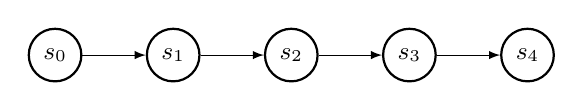
\begin{tikzpicture}[auto,node distance=15mm,>=latex,font=\small]
    \node[round] (s0) {$s_0$};
    \node[round, right of=s0] (s1) {$s_1$};
    \node[round, right of=s1] (s2) {$s_2$};
    \node[round, right of=s2] (s3) {$s_3$};
    \node[round, right of=s3] (s4) {$s_4$};

    \draw[->] (s0) -- (s1);
    \draw[->] (s1) -- (s2);
    \draw[->] (s2) -- (s3);
    \draw[->] (s3) -- (s4);
\end{tikzpicture}
\caption{Łańcuch Markova jako sieć przekonań}
\label{markov_chain}
\end{center}
\end{figure}
Rysunek \ref{markov_chain} pokazuje ogólny łańcuch Markova jako sieć przekonań.
Sieć ma pięć etapów, ale nie musi zatrzymywać się na $s_4$, może rozrastać
się w nieskończoność. Sieci przekonań przekazują założenie niezależności:
\[P(S_{i+1} | S_0, \dots , S_i) = P(S_{i+1} | S_i),\]
które jest nazywane \textbf{założeniem Markova}

Często sekwencje są rozłożone w czasie, wtedy $S_t$ reprezentuje stan w
momencie $t$. Intuicyjnie $S_t$ przekazuje całą informację o historii, która
mogłaby wpłynąć na przyszłe stany. Niezależność przypuszczenia w łańcuchu
Markova może być rozumiana jako ``biorąc pod uwagę teraźniejszość -- przyszłość
jest warunkowo niezależna od przeszłości''

Mówimy, że łańcuch Markova jest \textbf{modelem stacjonarnym} (ang.
\textit{stationary model}) oraz \textbf{czasowo homogenicznym modelem} (ang.
\textit{time-homogenous model}) jeżeli wszystkie zmienne mają tą samą dziedzinę
oraz wszystkie prawdopodobieństwa przejść są takie same dla każdego etapu, to
znaczy:
\[\forall i \ge 0, P(S_{i+1}|S_i) = P(S_1|S_0)\]
By określić stacjonarny łańcuch Markova, podano dwa prawdopodobieństwa
warunkowe:
\begin{itemize}
		\setlength\itemsep{-0.4em}
	\item $P(S_0)$ specyfikuje wszystkie początkowe warunki
	\item $P(S_{i+1} | S_i)$ specyfikuje \textbf{dynamikę}, która jest taka
		sama dla każdego $i \ge 0$
\end{itemize}
Stacjonarne łańcuchy Markova interesują nas z kilku względów:
\begin{itemize}
		\setlength\itemsep{-0.4em}
	\item Zapewniają prosty model, który jest łatwy do określenia
	\item Założenie stacjonarności jest często naturalnym modelem, ponieważ
		dynamika środowiska zazwyczaj nie zmienia się w czasie.
	\item Sieć może się rozrastać w nieskończoność. Określenie małej liczby
		parametrów daje nam nieskończoną
		sieć\cite{ai_foundations_markov_chains}.
\end{itemize}

% http://artint.info/2e/html/ArtInt2e.Ch9.S5.html
\subsection{Proces decyzyjny Markova}
Proces decyzyjny Markova, może być rozumiany jako łańcuch Markova powiększony o
działania agenta oraz nagrodę dla agenta. W każdym etapie agent decyduje jakie
działanie podjąć, nagroda i nowy stan zależą od podjętego przez agenta
działania oraz poprzedniego stanu. 

Rozważę jedynie stacjonarne modele łańcuchu Markova, gdzie przejścia między
stanami oraz nagrody nie zależą od czasu. 

Proces decyzyjny Markova (ang. \textit{Markov decision process (MDP)}) składa
się z:
\begin{itemize}
		\setlength\itemsep{-0.4em}
	\item $S$ -- zbiór stanów środowiska
	\item $A$ -- zbiór decyzji (akcji możliwych do podjęcia przez agenta)
	\item $P: S\times S\times A\rightarrow [0,1]$ -- funkcja, która określa
		\textbf{dynamikę}. Zapis $P(s' | s, a)$ oznacza
		prawdopodobieństwo, że agent przejdzie do stanu $s'$ pod
		warunkiem, że był w stanie $s$ i podjął akcję $a$, czyli:
		\[\forall s\in S \ \forall a\in A \sum_{s' \in S}P(s'|s,a)=1\]
	\item $R:S\times S\times A\times S \rightarrow \mathfrak{R}$, gdzie
		$R(s,a,s')$ to \textbf{funkcja nagrody}, dająca oczekiwaną
		natychmiastową nagrodę za wykonanie działania $a$ i przejścia
		do stanu $s'$ ze stanu $s$. Czasem wygodnie jest użyć zapisu
		$R(s,a)$ -- oczekiwana wartość wykonania $a$ w stanie $s$,
		która równa jest $R(s,a)=\sum _{s'}R(s,a,s') * P(s'|s,a)$.
\end{itemize}
\section{Q\dywiz learning}
Tutaj wszystko związane z qlearningiem, wzory, itp :)

\chapter{Implementacja Q\dywiz learningu}
\label{chapter:implementacja_qlearningu}
Tutaj fragmenty kodu, jakie zmiany dokonałem względem książkowego algorytmu
\section{Podejście pierwsze grid 10 na 10}
Po kolei wyjaśnienie co to grid 10 na 10 jak to jest implementowane itp
\section{Podejście drugie grid 10 na 10 i flaga za śmierć od wysokiej rury}
Jak wyżej
\section{Podejście trzecie grid 5 na 5 z flagą}
Jak wyżej

\chapter{Podsumowanie}
Wyniki osiągane są w miarę ok ale mogło by być lepiej bo są na internecie lepsze
podejścia do tego problemu -- być może wynika to z tego ze sam implementowałem grę
i nie jest ona tak dobrze przetestowana jak ta dostępna na GitHub?
\section{Co można by ulepszyć}
Tutaj będę pisał co mogłem zrobić gdybym poświęcił więcej czasu np:
\begin{itemize}
\item uczenie bez wizualizacji pygamowej
\item zrównoleglenie by paru agentów na raz mogło się uczyć
\item doszlifowanie algorytmu??
\end{itemize}


\addcontentsline{toc}{chapter}{Bibliografia}
\bibliographystyle{IEEEtran}
\bibliography{praca_licencjacka}

\end{document}
